\documentclass[tikz,border=4pt]{standalone}
\usepackage{fontspec}\usepackage{xcolor}\usetikzlibrary{arrows.meta,positioning,matrix}
\setsansfont{Lato}
\begin{document}
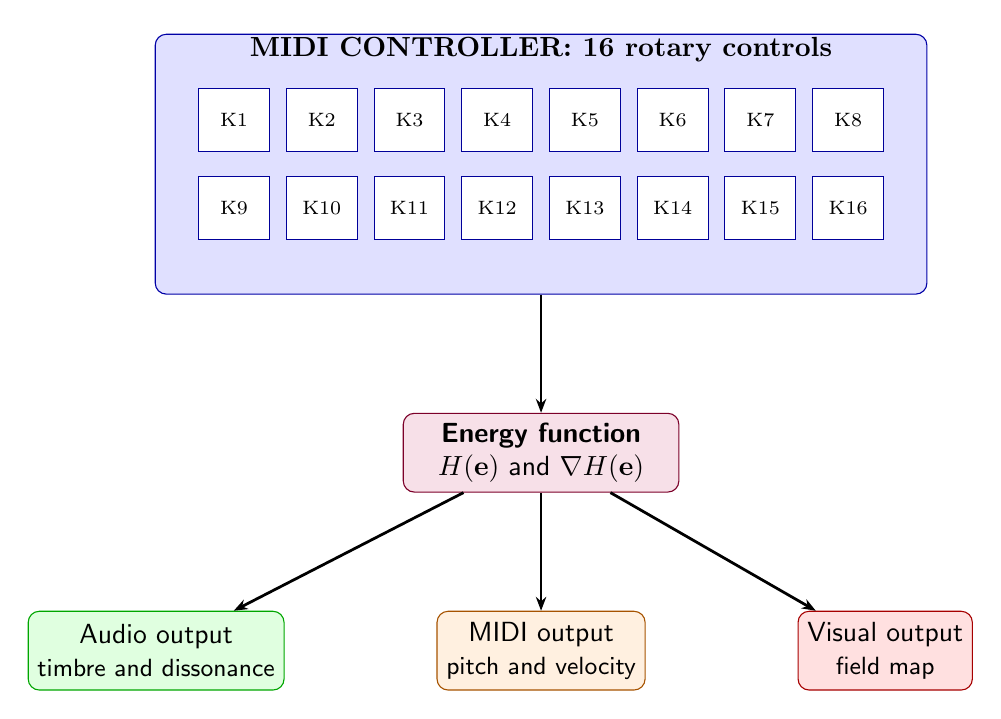
\begin{tikzpicture}[font=\sffamily,box/.style={rounded corners=4pt,draw=#1!65!black,fill=#1!12,align=center,minimum height=1cm},arrow/.style={-{Stealth[length=5pt]},line width=1pt}]
\node[box=blue,minimum width=9.8cm,minimum height=3.3cm] (midi) {};
\node[above=1.18cm of midi.center,font=\bfseries] {MIDI CONTROLLER: 16 rotary controls};
\matrix[matrix of nodes,nodes={draw=blue!60!black,fill=white,minimum width=9mm,minimum height=8mm,font=\scriptsize},column sep=2mm,row sep=3mm] at (midi.center) {K1 & K2 & K3 & K4 & K5 & K6 & K7 & K8\\K9 & K10 & K11 & K12 & K13 & K14 & K15 & K16\\};
\node[box=purple,below=1.5cm of midi,minimum width=3.5cm] (energy) {\textbf{Energy function}\\$H(\mathbf e)$ and $\nabla H(\mathbf e)$};
\draw[arrow] (midi) -- (energy);
\node[box=green,below left=1.5cm and 1.5cm of energy] (audio) {Audio output\\\small timbre and dissonance};
\node[box=orange,below=1.5cm of energy] (midiout) {MIDI output\\\small pitch and velocity};
\node[box=red,below right=1.5cm and 1.5cm of energy] (visual) {Visual output\\\small field map};
\draw[arrow] (energy) -- (audio);\draw[arrow] (energy) -- (midiout);\draw[arrow] (energy) -- (visual);
\end{tikzpicture}\end{document}
